\section{Overview}\label{sec:overview}
What we explore is the impact of different augmentations of the original data on the different dimensionality reduction techniques, and how this affects the performance of the \gls{ml} models.


\begin{description}
    \setlength\itemsep{0em}
    \item[dataset] mnist
    \item[pre-preprocessing] normalization, data augmentation
    \item[preprocessing] linear and non linear dimensionality reduction (PCA, LDA, Kernel PCA, and ISOMAP)
    \item[models] logistic regression and CNN
    \item[evaluation] accuracy, precision, recall, f1-score, speed/run time, memory usage, and model size
\end{description}


\subsection{Data collection}\label{subsec:data-collection}
The data used is the \gls{mnist} database, which is a collection of handwritten digits. The data is split into a training set of 60,000 images and a test set of 10,000 images. The images are 28x28 pixels, and each pixel is represented by a value between 0 and 255, where 0 is black and 255 is white. The images are grayscale, and the values are the intensity of the pixel. The images are labeled with the digit they represent, and the labels are integers between 0 and 9.

\subsection{Data pre-preprocessing}\label{subsec:data-pre-preprocessing}
The data is normalized by dividing each pixel value by 255, so that the values are between 0 and 1. The data is then augmented by rotating the images by 90, 180 and 270 degrees, and flipping the images horizontally and vertically. This results in 10 times as much data as the original \gls{mnist} dataset.\supervisor{This is just placeholder, but something like this is what we want to do.}

\subsection{Data preprocessing}\label{subsec:data-preprocessing}
The data is then preprocessed by applying linear and non-linear dimensionality reduction techniques. The linear dimensionality reduction techniques are \gls{pca} and \gls{lda}. The non-linear dimensionality reduction techniques are \gls{kpca} and \gls{isomap}. The data is reduced to 2 dimensions, so that it can be visualized.

\subsection{Model training}\label{subsec:model-training}
The \gls{lr} and \gls{cnn} models are then trained on both the original and the preprocessed data. The \gls{lr} model is trained\question{implemented?} using the \gls{sklearn} library, and the \gls{cnn} model is trained using the Keras library.\question{Maybe openCV library instead?}

\subsection{Evaluation}\label{subsec:evaluation}
The models are evaluated on the test set, and the results are compared. The evaluation metrics are accuracy, precision, recall, f1-score, speed/run time, memory usage, and model size. The results are visualized using graphs and tables, and presented in the results chapter.\question{Do we want to compare our results to the results of other papers?}

\todo[inline]{Explain the different evaluation metrics and how they are calculated and used to evaluate the effects of the different dimensionality reduction techniques. Perhaps write about why they were chosen, but maybe this is part of the problem analysis instead.}





An automation pipeline is created based on the model in Figure~\ref{fig:python-pipeline-model}.


\begin{figure}[htb!]
    \centering
    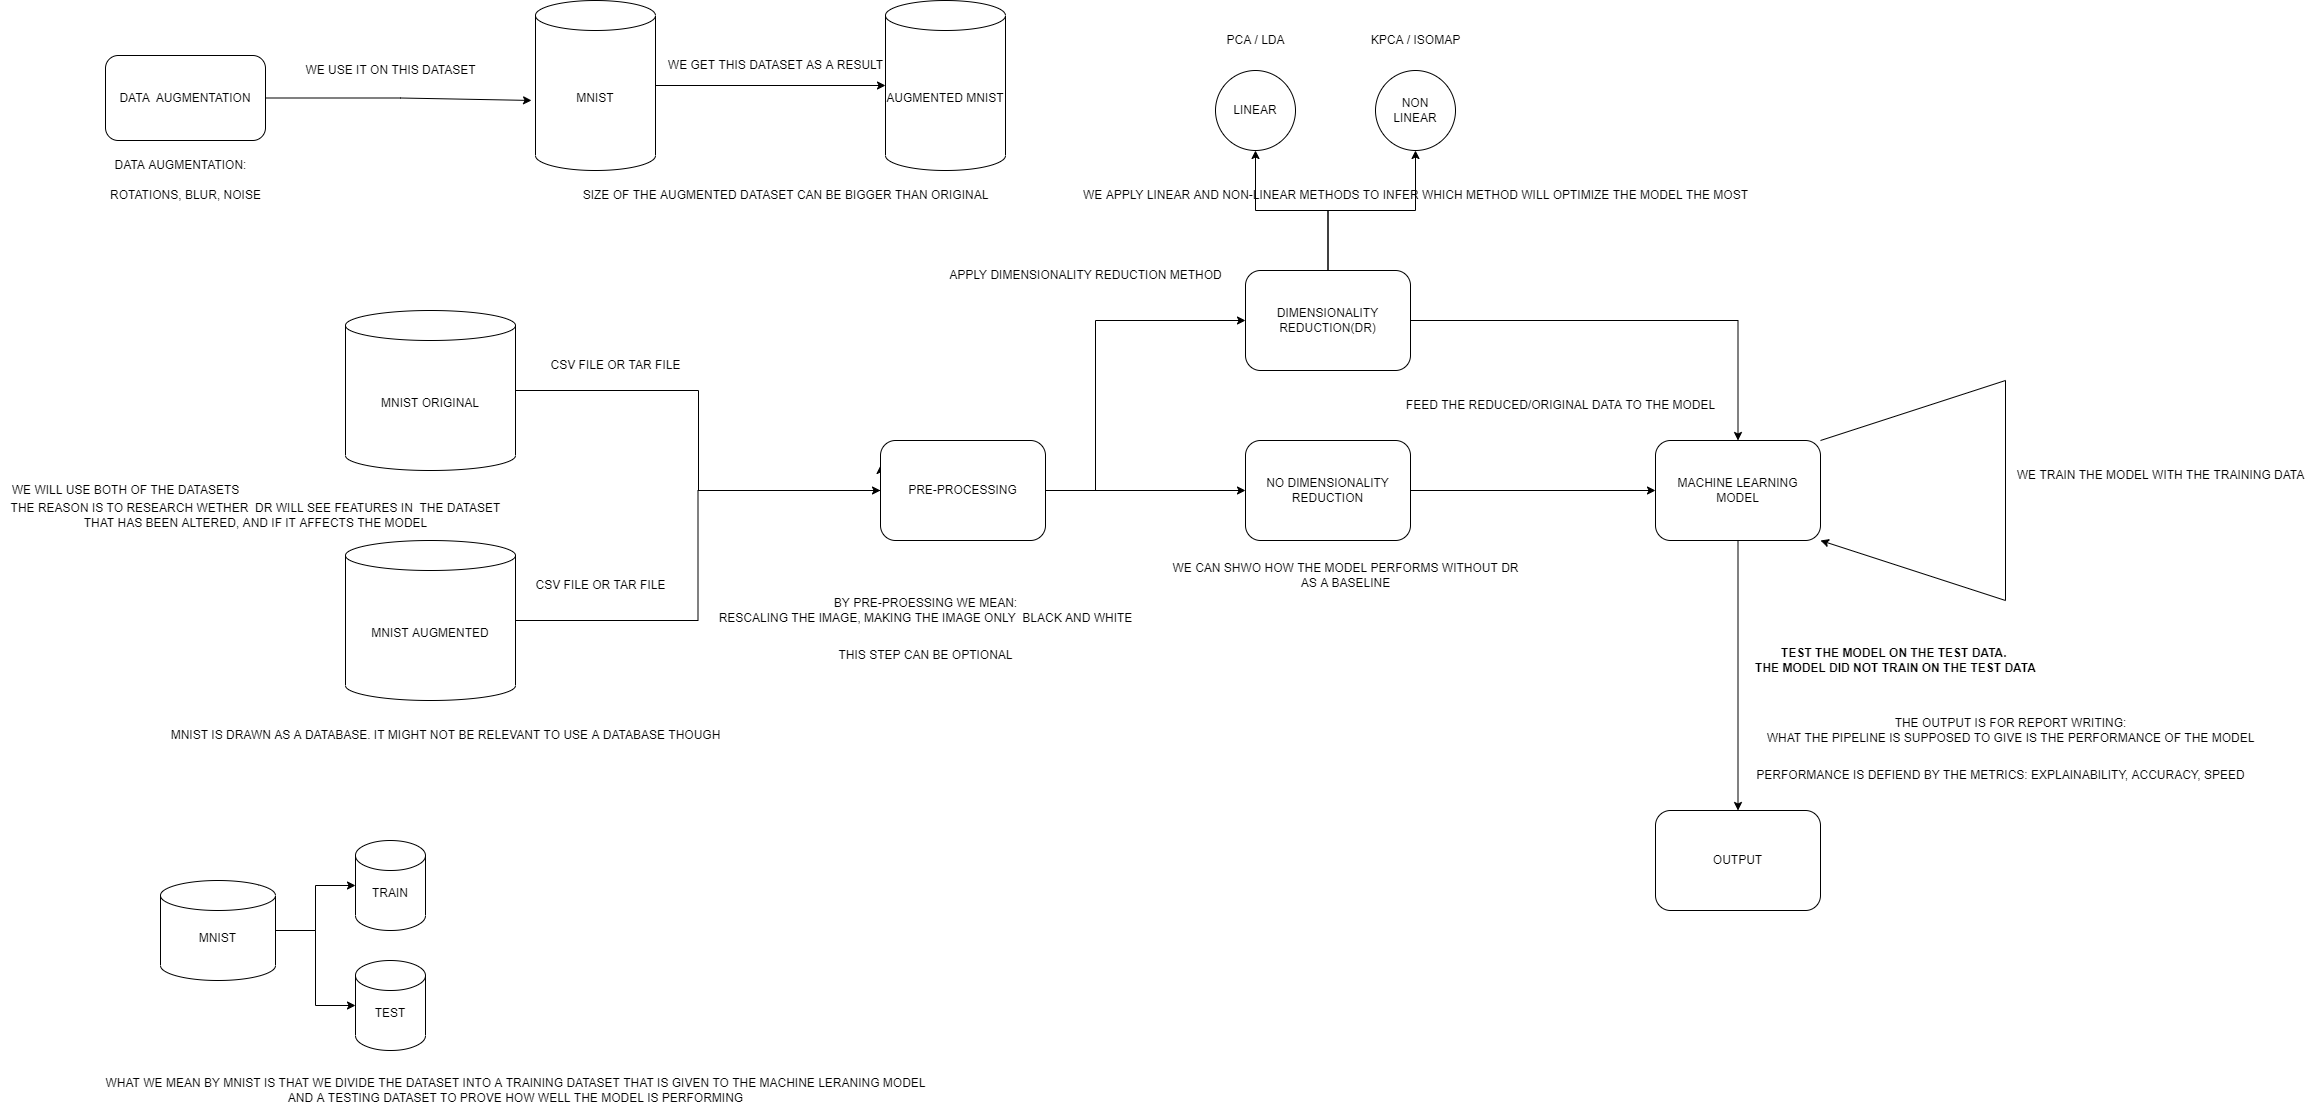
\includegraphics[width=\textwidth]{figures/pipeline-draft.png}
    \caption{Python project pipeline model.}
    \label{fig:python-pipeline-model}
\end{figure}


\urgent[inline]{write about the pipeline}
